\documentclass[twoside,11pt]{homework}

\coursename{EECS E6892 Fall 2015} % DON'T CHANGE THIS

\studentname{Daniel Kronovet}       % YOUR NAME GOES HERE
\studentmail{dbk2123@columbia.edu}   % YOUR UNI GOES HERE
\homeworknumber{3}               % THE HOMEWORK NUMBER GOES HERE
\collaborators{mkt2126, jma2215, psb2134}             % THE UNI'S OF STUDENTS YOU DISCUSSED WITH

\begin{document}
\maketitle

\section*{Problem 1}

\textbf{Part A}

Recall some basic rules of probability:

\[
p(\theta | x)p(x) = p(x, \theta)
\]

\[
p(x) = \frac{p(x, \theta)}{p(\theta | x)}
\]

\[
lnp(x) = lnp(x, \theta) - lnp(\theta | x)
\]

Note that:

\[
\int q(\theta) d\theta = 1
\]

Therefore:

\[
lnp(x) = lnp(x, \theta)\int q(\theta) d\theta - lnp(\theta | x)\int q(\theta) d\theta
\]

\[
lnp(x) = \int q(\theta) lnp(x, \theta) d\theta - \int q(\theta) lnp(\theta | x) d\theta
\]

We then add and subtract the entropy of $q(\theta)$:

\[
lnp(x) = \int q(\theta) lnp(x, \theta) d\theta - \int q(\theta) lnp(\theta | x) d\theta
+ \int q(\theta) lnq(\theta) d\theta - \int q(\theta) lnq(\theta) d\theta
\]

And reorganize:

\[
lnp(x) = \int q(\theta) (lnp(x, \theta) - q(\theta))d\theta - \int q(\theta) (lnp(\theta | x) - lnq(\theta)) d\theta
\]

\[
lnp(x) = \int q(\theta) ln\frac{p(x, \theta)}{q(\theta)} d\theta
 + \int q(\theta) ln\frac{q(\theta)}{p(\theta | x)} d\theta
\]

Having derived the VI master equation, we replace the generic $x$ with our data $x, y$ and the generic $q(\theta)$ with our variables $w, \lambda, \alpha$:

\[
lnp(y, x) = 
\int q(w, \lambda, \alpha) ln \frac{p(x,y,w, \lambda, \alpha)}{q(w, \lambda, \alpha)} dw d\lambda d\alpha
+ \int q(w, \lambda, \alpha) ln \frac{q(w, \lambda, \alpha)}{p(w, \lambda, \alpha | x, y} dw d\lambda d\alpha
\]

We define $q(w, \lambda, \alpha) = q(w)q(\lambda)q(\alpha)$:

\begin{equation}
lnp(y, x) = 
\underbrace{
\int q(w)q(\lambda)q(\alpha) ln \frac{p(x,y,w, \lambda, \alpha)}{q(w)q(\lambda)q(\alpha)} dw d\lambda d\alpha
}_{\cL}
+ \underbrace{
\int q(w)q(\lambda)q(\alpha) ln \frac{q(w)q(\lambda)q(\alpha)}{p(w, \lambda, \alpha | x, y} dw d\lambda d\alpha
}_{KL(q||p)}
\end{equation}

We will reference this equation throughout the derivation.

We turn to $\cL$, and observe that it can be rewritten as follows:

\[
\cL =
\int q(w)q(\lambda)q(\alpha) ln p(x,y,w, \lambda, \alpha) dw d\lambda d\alpha
- \int q(w)q(\lambda)q(\alpha) lnq(w)q(\lambda)q(\alpha) dw d\lambda d\alpha
\]

\begin{equation}
\cL =
\int q(w)q(\lambda)q(\alpha) ln p(x,y,w, \lambda, \alpha) dw d\lambda d\alpha
- \int q(w)lnq(w)dw
- \int q(\lambda)lnq(\lambda)d\lambda
- \int q(\alpha)lnq(\alpha) d\alpha
\end{equation}

Now, WLOG, observe that for variable $w$:

\[
\cL =
\int q(w)
\Brackets{ \int
q(\lambda)q(\alpha) ln p(x,y,w, \lambda, \alpha) d\lambda d\alpha
} dw
- \int q(w)lnq(w)dw
- (\text{const w.r.t.} w)
\]

\[
\cL =
\int q(w)
\bbE_{-q(w)} \Brackets{
ln p(x,y,w, \lambda, \alpha)
} dw
- \int q(w)lnq(w)dw
- (\text{const w.r.t.} w)
\]

Then, we introduce $Z$ as shown in class:

\[
\cL =
\int q(w) ln \frac{1}{Z}e^{
\bbE \Brackets{
ln p(x,y,w, \lambda, \alpha)
}} dw
- \int q(w)lnq(w)dw
- lnZ - (\text{const w.r.t.} w)
\]

As $Z$ is an integral over $w$, it is constant w.r.t $w$. Therefore we can roll $-lnZ$ into the constant.

\[
\cL =
\underbrace{
\int q(w) ln \frac{\frac{1}{Z} e^{
\bbE \Brackets{
ln p(x,y,w, \lambda, \alpha)
}}}{
q(w)
} dw
}_{-KL(q||p)}
- (\text{const w.r.t.} w)
\]

We seek to maximize this expression. $KL$ is minimized (and therefore $-KL$ is maximized) when the the two distributions are equal. Therefore, for each variable, we will set:

\[
q = \frac{1}{Z} e^{
\bbE \Brackets{
ln p(x,y,w, \lambda, \alpha)
}}
\]

Evaluated for each variable, using the expectation over all other variables.

First, we will write out the log joint likelihood and the individual likelihoods, for reference:

\[
ln p(x,y,w, \lambda, \alpha) = 
ln p(y | x, w, \lambda) + ln p(w | \alpha) + ln p(\lambda | e_0, f_0) + ln p(\alpha | a_0, b_0)
\]

\begin{equation}
ln p(x,y,w, \lambda, \alpha) = 
 \sum_{i=1}^n  ln p(y_i | x_i, w, \lambda) + ln p(w | \alpha)
+ ln p(\lambda | e_0, f_0) + \sum_{k=1}^d ln p(\alpha_k | a_0, b_0)
\end{equation}

\begin{equation}
 \sum_{i=1}^n  ln p(y_i | x_i, w, \lambda) = 
 \frac{n}{2}ln\lambda - \frac{n}{2}ln2\pi - \frac{\lambda}{2} \sum_{i=1}^n(y_i^2 - 2w^Tx_iy_i + w^Tx_ix_i^Tw)
\end{equation}

\begin{equation}
ln p(w | \alpha) =
 \frac{1}{2}\sum_{k=1}^dln\alpha_k - \frac{1}{2}ln2\pi - \frac{1}{2}(w^Tdiag(\alpha_j)w)
\end{equation}

\begin{equation}
ln p(\lambda | e_0, f_0) =
e_0lnf_0 - ln\Gamma(e_0) + (e_0 - 1)ln\lambda - f_0\lambda
\end{equation}

\begin{equation}
ln p(\alpha_k | a_0, b_0) =
a_0lnb_0 - ln\Gamma(a_0) + (a_0 - 1)ln\alpha_k - b_0\alpha_k
\end{equation}

Now, we will begin with $w$:

\[
\bbE_{-q(w)} \Brackets{
 \sum_{i=1}^n  ln p(y_i | x_i, w, \lambda) + ln p(w | \alpha)
+ ln p(\lambda | e_0, f_0) + \sum_{k=1}^d ln p(\alpha_k | a_0, b_0)
}
\]

First, we can disregard all terms not involving $w$, as they will be absorbed into the normalizing constant.

\[
\bbE_{-q(w)} \Brackets{
 \sum_{i=1}^n  ln p(y_i | x_i, w, \lambda) + ln p(w | \alpha)
}
\]

Plugging in the distributions:

\[
\bbE_{-q(w)} \Brackets{
 \frac{n}{2}ln\lambda - \frac{n}{2}ln2\pi - \frac{\lambda}{2} \sum_{i=1}^n(y_i^2 - 2w^Tx_iy_i + w^Tx_ix_i^Tw)
 +  \frac{1}{2}\sum_{k=1}^dln\alpha_k - \frac{1}{2}ln2\pi - \frac{1}{2}(w^Tdiag(\alpha_j)w)
}
\]

Disregarding additional terms not in $w$:

\[
\bbE_{-q(w)} \Brackets{
- \frac{\lambda}{2} \sum_{i=1}^n(y_i^2 - 2w^Tx_iy_i + w^Tx_ix_i^Tw)
 - \frac{1}{2}(w^Tdiag(\alpha_j)w)
}
\]

\[
\bbE_{-q(w)} - \frac{1}{2}  \Brackets{
\lambda \sum_{i=1}^n(y_i^2 - 2w^Tx_iy_i + w^Tx_ix_i^Tw)
+ (w^Tdiag(\alpha_j)w)
}
\]

Now, we pass the expectation through. Recall, this is an expectation over $\lambda, \alpha$:

\[
- \frac{1}{2}  \Brackets{
\bbE\lambda \sum_{i=1}^n(y_i^2 - 2w^Tx_iy_i + w^Tx_ix_i^Tw)
+ (w^T\bbE[diag(\alpha_j)]w)
}
\]

Now we must complete the square to solve for $w$. This is a procedure we are becoming familiar with.

\[
- \frac{1}{2}  \Brackets{
w^T\Parens{\bbE[diag(\alpha_j)] + \bbE \lambda \sum x_ix_i^T}w
- 2w^T\Parens{\bbE \lambda \sum x_iy_i}
+ \bbE \lambda \sum y_i^2
}
\]

We drop the rightmost term.

\[
- \frac{1}{2}  \Brackets{
w^T\Parens{\bbE[diag(\alpha_j)] + \bbE \lambda \sum x_ix_i^T}w
- 2w^T\Parens{\bbE \lambda \sum x_iy_i}
}
\]

We then save time by shamelessly referring to our Lecture 2 notes for the final result:

\[
\Sigma^\prime = \Parens{\bbE[diag(\alpha)] + \bbE \lambda \sum_{i=1}^n x_i x_i^T}^{-1}
\]

\[
\mu^\prime = \Sigma^\prime \Parens{\bbE \lambda \sum_{i=1}^n y_i x_i}
\]

Therefore we set:

\begin{equation}
q(w) = N(\mu^\prime, \Sigma^\prime)
\end{equation}

Once we have $q(\lambda)$ and $q(\alpha)$ we will be able to evaluate these expressions exactly.

We repeat the process for $q(\lambda)$:

\[
\bbE_{-q(\lambda)} \Brackets{
 \sum_{i=1}^n  ln p(y_i | x_i, w, \lambda) + ln p(w | \alpha)
+ ln p(\lambda | e_0, f_0) + \sum_{k=1}^d ln p(\alpha_k | a_0, b_0)
}
\]


\[
\bbE_{-q(\lambda)} \Brackets{
\frac{n}{2}ln\lambda - \frac{n}{2}ln2\pi - \frac{\lambda}{2} \sum_{i=1}^n(y_i^2 - 2w^Tx_iy_i + x_i^Tww^Tx_i)
+ e_0lnf_0 - ln\Gamma(e_0) + (e_0 - 1)ln\lambda - f_0\lambda
}
\]

Tossing what is not in $\lambda$:

\[
\bbE_{-q(\lambda)} \Brackets{
\frac{n}{2}ln\lambda - \frac{\lambda}{2} \sum_{i=1}^n(y_i^2 - 2w^Tx_iy_i + x_i^Tww^Tx_i)
+ (e_0 - 1)ln\lambda - f_0\lambda
}
\]

Passing through the expectation (now over $w, \alpha$):

\[
\frac{n}{2}ln\lambda - \frac{\lambda}{2} \sum_{i=1}^n(y_i^2 - 2\bbE[w]^Tx_iy_i + x_i^T\bbE[ww^T]x_i)
+ (e_0 - 1)ln\lambda - f_0\lambda
\]

Rearranging, we recover a Gamma distribution in $\lambda$:

\[
ln\lambda \Parens{
\frac{n}{2} + e_0 - 1
} - \lambda\Parens{
\frac{1}{2} \sum_{i=1}^n(y_i^2 - 2\bbE[w]^Tx_iy_i + x_i^T\bbE[ww^T]x_i) + f_0
}
\]

With updated parameters:

\[
e^\prime = \frac{n}{2} + e_0
\]

\[
f^\prime = \frac{1}{2} \sum_{i=1}^n(y_i^2 - 2\bbE[w]^Tx_iy_i + x_i^T\bbE[ww^T]x_i) + f_0
\]

Which can be rewritten as:

\[
f^\prime = \frac{1}{2} \sum_{i=1}^n(y_i^2 - 2\mu^{\prime T} x_iy_i + x_i^T[ \Sigma^\prime + \mu^\prime \mu^{\prime T}]]x_i) + f_0
\]

\[
f^\prime = \frac{1}{2} \sum_{i=1}^n [(y_i - \mu^{\prime T}x_i)^2 + x_i^T\Sigma^\prime x_i] + f_0
\]

Thus, we set:

\begin{equation}
q(\lambda) = Gamma(e^\prime, f^\prime)
\end{equation}


We turn now to $q(\alpha)$. Recall that $\alpha = \alpha_i, ..., \alpha_d \stackrel{iid}{\sim} Gamma(a_0, b_0)$. Given their independence, we will solve for an arbitrary $\alpha_j$.

\[
\bbE_{-q(\alpha_j)} \Brackets{
 \sum_{i=1}^n  ln p(y_i | x_i, w, \lambda) + ln p(w | \alpha)
+ ln p(\lambda | e_0, f_0) + \sum_{k=1}^d ln p(\alpha_k | a_0, b_0)
}
\]

\[
\bbE_{-q(\alpha_j)} \Brackets{
ln p(w | \alpha)
+ ln p(\alpha_j | a_0, b_0)
}
\]

\[
\bbE_{-q(\alpha_j)} \Brackets{
 \frac{1}{2}\sum_{k=1}^dln\alpha_k - \frac{1}{2}ln2\pi - \frac{1}{2}(w^Tdiag(\alpha)w)
+ a_0lnb_0 - ln\Gamma(a_0) + (a_0 - 1)ln\alpha_j - b_0\alpha_j
}
\]

\[
\bbE_{-q(\alpha_j)} \Brackets{
 \frac{1}{2}ln\alpha_j - \frac{1}{2}(w^Tdiag(\alpha)w)
+ (a_0 - 1)ln\alpha_j - b_0\alpha_j
}
\]

We pass the expectation through (over $w, \lambda, \alpha_{k \neq j}$).

\[
 \frac{1}{2}ln\alpha_j - \frac{1}{2}\bbE[w^Tdiag(\alpha)w]
+ (a_0 - 1)ln\alpha_j - b_0\alpha_j
\]

We can rewrite the expectation as follows:

\[
\bbE[w^Tdiag(\alpha)w] =
\sum_{k=1}^d \bbE[w_k^2] \alpha_k
\]

As a summation over all $\alpha$, we observe we can discard all terms where $\alpha_{k \neq j}$, leaving us with:

\[
 \frac{1}{2}ln\alpha_j - \frac{1}{2}\bbE[w_j^2] \alpha_j
+ (a_0 - 1)ln\alpha_j - b_0\alpha_j
\]

From here, we recover a Gamma distribution in $\alpha_j$:

\[
 ln\alpha_j (\frac{1}{2} + a_0 - 1)
 - \alpha_j(\frac{1}{2}\bbE[w_j^2] + b_0)
\]

Thus, we set:

\[
a^\prime = (a_0 + \frac{1}{2})
\]

\[
b^\prime = (b_0 + \frac{1}{2}\bbE[w_j^2])
\]

\begin{equation}
q(\alpha_j) = Gamma(a^\prime, b^\prime)
\end{equation}

To finish the derivations, we observe that we must evaluate the following expectations:
$\bbE[\lambda], \bbE[w], \bbE[ww^T], \bbE[w_j^2], \bbE[diag(\alpha)]$.

With our distributions as derived, we have:

\[
\bbE[\lambda] = \frac{e^\prime}{f^\prime}
\]

For $\bbE[diag(\alpha)]$, we observe that each $\alpha$ is independent. Thus it suffices to find $\bbE[\alpha_k]$.

\[
\bbE[\alpha_k] = \frac{a^\prime_k}{b^\prime_k}
\]

The next expectation is straightforward:

\[
\bbE[w] = \mu^\prime
\]

The remaining two expectations require some more work:

\[
cov(w) = \bbE[ww^T] - \mu^\prime \mu^{\prime T}
\]

\[
\bbE[ww^T] = cov(w) + \mu^\prime \mu^{\prime T}
\]

\[
\bbE[ww^T] = \Sigma^\prime + \mu^\prime \mu^{\prime T}
\]

From there, we can also observe:

\[
\bbE[w_j^2] = \bbE[ww^T] _{jj} = \Sigma^\prime_{jj} + [\mu^\prime \mu^{\prime T}]_{jj}
\]


\textbf{Part B}

For our algorithm, we review our results from Part A:

First, our input: data and the following definitions:

\[
q(w) = N(\mu^\prime, \Sigma^\prime)
\]

\[
q(\lambda) = Gamma(e^\prime, f^\prime)
\]

\[
q(\alpha_j) = Gamma(a^\prime, b^\prime)
\]

Our output will be a set of values for $\mu^\prime, \Sigma^\prime, e^\prime, f^\prime, a^\prime, b^\prime$.

To produce our output, we initialize our variable as follows:

\[
\mu^\prime_0 = \vec{0}
\]

\[
\Sigma^\prime_0 = diag\Parens{\frac{a_0}{b_0},...}^{-1}
\]

\[
e^\prime_0 = 1
\]

\[
f^\prime_0 = 1
\]

\[
a^\prime_0 = 10^{-16}
\]

\[
b^\prime_0 = 10^{-16}
\]

For iteration $t = 1, ..., T$:

1. Update $q_t(\alpha_k)$ for $k = 1, ..., d$ by setting:
	
\[
a^\prime_{kt} = (a_0 + \frac{1}{2})
\]

\[
b^\prime_{kt} = (b_0 + \frac{1}{2}([\Sigma^\prime_{t-1}]_{jj} + [\mu^\prime_{t-1} \mu^{\prime T}_{t-1}]_{jj}))
\]

2. Update $q_t(\lambda)$ by setting:

\[
e^\prime_t = \frac{n}{2} + e_0
\]

\[
f^\prime = \frac{1}{2} \sum_{i=1}^n [(y_i - \mu^{\prime T}_{t-1}x_i)^2 + x_i^T\Sigma^\prime_{t-1} x_i] + f_0
\]

3. Update $q_t(w)$ by setting:

\[
\Sigma^\prime_t = \Parens{diag(\frac{a^\prime_t}{b^\prime_t},...)] + \frac{e^\prime_t}{f^\prime_t} \sum_{i=1}^n x_i x_i^T}^{-1}
\]

\[
\mu^\prime_t = \Sigma^\prime_t \Parens{\frac{e^\prime_t}{f^\prime_t} \sum_{i=1}^n y_i x_i}
\]

Now, we evaluate $\cL(a^\prime_{t}, b^\prime_{t}, e^\prime_t, f^\prime_t, \mu^\prime_t, \Sigma^\prime_t)$ to assess convergence.

\textbf{Part C}

We now calculate $\cL$, the variational objective function. From equation 2, we have:

\[
\cL =
\int q(w)q(\lambda)q(\alpha) ln p(x,y,w, \lambda, \alpha) dw d\lambda d\alpha
- \int q(w)lnq(w)dw
- \int q(\lambda)lnq(\lambda)d\lambda
- \int q(\alpha)lnq(\alpha) d\alpha
\]

Which we interpret as:

\[
\cL =
\bbE_q [ln p(x,y,w, \lambda, \alpha) ]
- \bbE_q[lnq(w)]
- \bbE_q[lnq(\lambda)]
- \bbE_q[lnq(\alpha)]
\]

We are then interested in taking these expectations. Unlike the expectations we took for the $q$ distributions, these expectations are over all variables $w, \lambda, \alpha$.

\[
\cL =
\bbE_q [ln p(x,y,w, \lambda, \alpha) ]
- \bbE_q[lnq(w)]
- \bbE_q[lnq(\lambda)]
- \bbE_q[lnq(\alpha)]
\]

We expand the equation (which now spills onto two lines):

\[
\bbE_q [ \sum_{i=1}^n  ln p(y_i | x_i, w, \lambda)]
+ \bbE_q[ln p(\lambda | e_0, f_0)]
+ \bbE_q[ln p(w | \alpha)]
+ \bbE_q[ \sum_{k=1}^d ln p(\alpha_k | a_0, b_0)]
\]

\begin{equation}
- \bbE_q[lnq(w | \mu^\prime, \Sigma^\prime)]
- \bbE_q[lnq(\lambda | e^\prime, f^\prime)]
- \bbE_q[\sum_{k=1}^d lnq(\alpha | a^\prime, b^\prime)]
\end{equation}

Notice that the distributions form natural pairs. We will evaluate the pairs in turn.

First, we consider:

\[
\bbE[ ln p(\lambda | e_0, f_0)] - \bbE_q[lnq(\lambda | e^\prime, f^\prime)]
\]

\[
\bbE \Brackets{
(e_0lnf_0 - ln\Gamma(e_0) + (e_0 - 1)ln\lambda - f_0\lambda) -
(e^\prime lnf^\prime - ln\Gamma(e^\prime) + (e^\prime - 1)ln\lambda - f^\prime\lambda)
}
\]

Passing the expectations through:

\[
e_0lnf_0 - ln\Gamma(e_0) + (e_0 - 1)\bbE[ln\lambda] - f_0\bbE[\lambda] -
e^\prime lnf^\prime + ln\Gamma(e^\prime) - (e^\prime - 1)\bbE[ln\lambda] + f^\prime\bbE[\lambda]
\]

We know that $\bbE[\lambda] = \frac{e^\prime}{f^\prime}$. What about $\bbE[ln\lambda]$?
Looking up this expectation, we see that it is equal to $\psi(e^\prime) - lnf^\prime$, with $\psi$ representing the Digamma function.

Replacing the expectations with their values, we have:

\[
e_0lnf_0 - ln\Gamma(e_0) + (e_0 - 1)(\psi(e^\prime) - lnf^\prime) - f_0\frac{e^\prime}{f^\prime} -
e^\prime lnf^\prime + ln\Gamma(e^\prime) - (e^\prime - 1)(\psi(e^\prime) - lnf^\prime) + f^\prime\frac{e^\prime}{f^\prime}
\]

Simplifying:

\begin{equation}
(e_0lnf_0 - ln\Gamma(e_0)) - (e^\prime lnf^\prime + ln\Gamma(e^\prime))
+ (e_0 - e^\prime)(\psi(e^\prime) - lnf^\prime)
- (f_0 - f^\prime)\frac{e^\prime}{f^\prime}
\end{equation}

The first term in the objective function.

Then, we consider the related:

\[
\bbE[ \sum_{k=1}^d ln p(\alpha | a_0, b_0)] - \bbE_q[\sum_{k=1}^d lnq(\alpha | a^\prime, b^\prime)]
\]

\[
da_0lnb_0 - dln\Gamma(a_0) + (a_0 - 1)\sum_{k=1}^d \bbE[ln\alpha_k] - b_0\sum_{k=1}^d \bbE[\alpha_k]
- \sum_{k=1}^d \Brackets{
a^\prime lnb^\prime_k - ln\Gamma(a^\prime) + (a^\prime - 1)\bbE[ln\alpha_k] - b^\prime_k \bbE[\alpha_k]
}
\]

We evaluate $\bbE[\alpha_k]$ and $\bbE[ln\alpha_k]$ the same as before. The resulting expression takes two lines:

\[
da_0lnb_0 - dln\Gamma(a_0) + (a_0 - 1)\sum_{k=1}^d (\psi(a^\prime) - lnb^\prime_k) - b_0\sum_{k=1}^d \frac{a^\prime}{b^\prime_k}
\]

\[
- \sum_{k=1}^d \Brackets{
a^\prime lnb^\prime_k - ln\Gamma(a^\prime)
+ (a^\prime - 1)(\psi(a^\prime) - lnb^\prime_k)
- b^\prime_k \frac{a^\prime}{b^\prime_k}
 } 
\]

Which can be simplified:

\begin{equation}
d(a_0lnb_0 - ln\Gamma(a_0)) - (a^\prime \sum_{k=1}^d lnb^\prime_k - dln\Gamma(a^\prime))
+ (a_0 - a^\prime)\sum_{k=1}^d \Brackets{(\psi(a^\prime) - lnb^\prime_k)}
- b_0\sum_{k=1}^d \Brackets{\frac{a^\prime}{b^\prime_k}} + da^\prime
\end{equation}

Then, we evaluate:

\[
\bbE_q[ln p(w | \alpha)]
- \bbE_q[lnq(w | \mu^\prime, \Sigma^\prime)]
\]

\[
 \frac{1}{2}\sum_{k=1}^d \bbE[ln\alpha_k] - \frac{d}{2}ln2\pi - \frac{1}{2}(\bbE[w^Tdiag(\alpha)]w])
 + \frac{1}{2}ln|[\Sigma^\prime| + \frac{k}{2}ln2\pi + \frac{1}{2}\bbE[(w - \mu^\prime)^T\Sigma^{\prime -1}(w - \mu^\prime)]
\]

Taking the same sorts of expectations, we see that $\bbE[ln\alpha_{0k}] = \psi(a^\prime_{0k}) - lnb^\prime_{0k}$.
Recall also that:

\[
\bbE[w^Tdiag(\alpha)w]
= \sum_{k=1}^d \bbE[w_k^2] \bbE[\alpha_k]
= \sum_{k=1}^d [\Sigma^\prime_{kk} + [\mu^\prime \mu^{\prime T}]_{kk}]\frac{a^\prime}{b^\prime_k}
\]

Regarding $\bbE[(w - \mu^\prime)^T\Sigma^{\prime -1}(w - \mu^\prime)]$, observe that:

\[
\bbE[(w - \mu^\prime)^T\Sigma^{\prime -1}(w - \mu^\prime)]
\]

\[
\bbE[w^T \Sigma^{\prime -1}w]
- 2\bbE[w]\Sigma^{\prime -1} \mu^\prime
+ \mu^{\prime T}\Sigma^{\prime -1} \mu^\prime
\]

\[
\bbE[w^T \Sigma^{\prime -1}w]
- \mu^{\prime T}\Sigma^{\prime -1} \mu^\prime
\]

We use the trace rule $uv^T = tr(u^Tv)$ and the symmetry of $\Sigma^\prime$:

\[
\bbE[tr(\Sigma^{\prime -1}ww^T)]
- tr(\Sigma^{\prime -1} \mu^\prime \mu^{\prime T})
\]

\[
tr(\Sigma^{\prime -1} \bbE[ww^T])
- tr(\Sigma^{\prime -1} \mu^\prime \mu^{\prime T})
\]

\[
\sum_{k=1}^d \Brackets{
\Sigma^{\prime -1}_{kk} (
\bbE[ww^T]_{kk}
- [\mu^\prime \mu^{\prime T}]_{kk}
)}
\]

\[
\sum_{k=1}^d \Brackets{
\Sigma^{\prime -1}_{kk} (
\Sigma^\prime_{kk} + [\mu^\prime \mu^{\prime T}]_{kk}
- [\mu^\prime \mu^{\prime T}]_{kk}
)}
\]

\[
\sum_{k=1}^d \Brackets{
\Sigma^{\prime -1}_{kk} \Sigma^\prime_{kk}}
\]

\[
\sum_{k=1}^d \Brackets{1} = d
\]

Returning to $lnp(w)$ and $lnq(w)$:

\[
 \frac{1}{2}\sum_{k=1}^d \bbE[ln\alpha_k] - \frac{d}{2}ln2\pi - \frac{1}{2}(w^T\bbE[diag(\alpha)]w)
 + \frac{1}{2}ln|[\Sigma^\prime| + \frac{d}{2}ln2\pi + \frac{1}{2}(w - \mu^\prime)^T\Sigma^{\prime -1}(w - \mu^\prime)
\]

We plug in the expectations:

\[
 \frac{1}{2}\sum_{k=1}^d (\psi(a^\prime) - lnb^\prime_k) - \frac{d}{2}ln2\pi -
 \frac{1}{2}\sum_{k=1}^d \Brackets{[\Sigma^\prime_{kk} + [\mu^\prime \mu^{\prime T}]_{kk}]\frac{a^\prime}{b^\prime_k}}
+ \frac{1}{2}ln|[\Sigma^\prime| + \frac{d}{2}ln2\pi + \frac{d}{2}
\]

Dropping constant terms:

\begin{equation}
 \frac{1}{2}\sum_{k=1}^d (\psi(a^\prime_k) - lnb^\prime_k)
 - \frac{1}{2}\sum_{k=1}^d \Brackets{[\Sigma^\prime_{kk} + [\mu^\prime \mu^{\prime T}]_{kk}]\frac{a^\prime}{b^\prime_k}}
+ \frac{1}{2}ln|\Sigma^\prime|
\end{equation}


Lastly, we evaluate:

\[
\bbE_q [ \sum_{i=1}^n  ln p(y_i | x_i, w, \lambda)]
\]

\[
\frac{n}{2}\bbE [ln\lambda] - \frac{n}{2}ln2\pi - \frac{\bbE [\lambda]}{2} \sum_{i=1}^n (y_i^2 - 2\bbE [w]^Tx_iy_i + x_i^T\bbE [ww^T]x_i)]
\]

\[
\frac{n}{2}(\psi(e^\prime) - lnf^\prime) - \frac{n}{2}ln2\pi - \frac{f^\prime_k}{2e^\prime_k} \sum_{i=1}^n (y_i^2 - 2\mu^{\prime T}x_iy_i + x_i^T [\Sigma^\prime + \mu^\prime \mu^{\prime T}]x_i)]
\]

Again, dropping constant terms:

\begin{equation}
\frac{n}{2}(\psi(e^\prime) - lnf^\prime)
- \frac{f^\prime}{2e^\prime} \sum_{i=1}^n \Brackets{y_i^2 - 2\mu^{\prime T}x_iy_i + x_i^T [\Sigma^\prime + \mu^\prime \mu^{\prime T}]x_i}
\end{equation}

We now present the full variational inference objective function, less the constant terms. This is the expression we will evaluate to assess convergence.

\[
(e_0lnf_0 - ln\Gamma(e_0)) - (e^\prime lnf^\prime + ln\Gamma(e^\prime))
+ (e_0 - e^\prime)(\psi(e^\prime) - lnf^\prime)
- (f_0 - f^\prime)\frac{e^\prime}{f^\prime}
\]

\[
d(a_0lnb_0 - ln\Gamma(a_0)) - (a^\prime \sum_{k=1}^d lnb^\prime_k - dln\Gamma(a^\prime))
+ (a_0 - a^\prime)\sum_{k=1}^d \Brackets{(\psi(a^\prime) - lnb^\prime_k)}
- b_0\sum_{k=1}^d \Brackets{\frac{a^\prime}{b^\prime_k}} + da^\prime
\]

\[
 \frac{1}{2}\sum_{k=1}^d (\psi(a^\prime_k) - lnb^\prime_k)
 - \frac{1}{2}\sum_{k=1}^d \Brackets{[\Sigma^\prime_{kk} + [\mu^\prime \mu^{\prime T}]_{kk}]\frac{a^\prime}{b^\prime_k}}
+ \frac{1}{2}ln|\Sigma^\prime|
\]

\begin{equation}
+ \frac{n}{2}(\psi(e^\prime) - lnf^\prime)
- \frac{f^\prime}{2e^\prime} \sum_{i=1}^n \Brackets{y_i^2 - 2\mu^{\prime T}x_iy_i + x_i^T [\Sigma^\prime + \mu^\prime \mu^{\prime T}]x_i}
\end{equation}

\section*{Problem 2}

As an aid to implementation, we observe that, for invertible matrix $A \in R^{n \times n}$, we can decompose $A = LL^T$ (the Cholesky decomposition).
Note that for complex-valued matrices, we would use $L^*$, the conjugate transpose instead of $L^T$.

Therefore, $A^{-1} = L^{-1}L^{-1T}$. In regards to determinants, we know that $|AB| = |A||B|$. Therefore, we can say that:

\[
|A^{-1}| = |L^{-1}||L^{-1T}|
\]

The determinant of a triangular matrix is the product of the diagonal terms:

\[
|L^{-1}||L^{-1T}| = \prod_{i=1}^n L^{-1}_{ii}    \prod_{i=1}^n L^{-1T}_{ii}
\]

The log determinant is therefore a summation over the log of the diagonal:

\[
ln[|L^{-1}||L^{-1T}|] = \sum_{i=1}^n lnL^{-1}_{ii}  +  \sum_{i=1}^n lnL^{-1T}_{ii} = 2\sum_{i=1}^n lnL^{-1}_{ii}
\]

\textbf{N = 100}

a. Variational Objective Function:

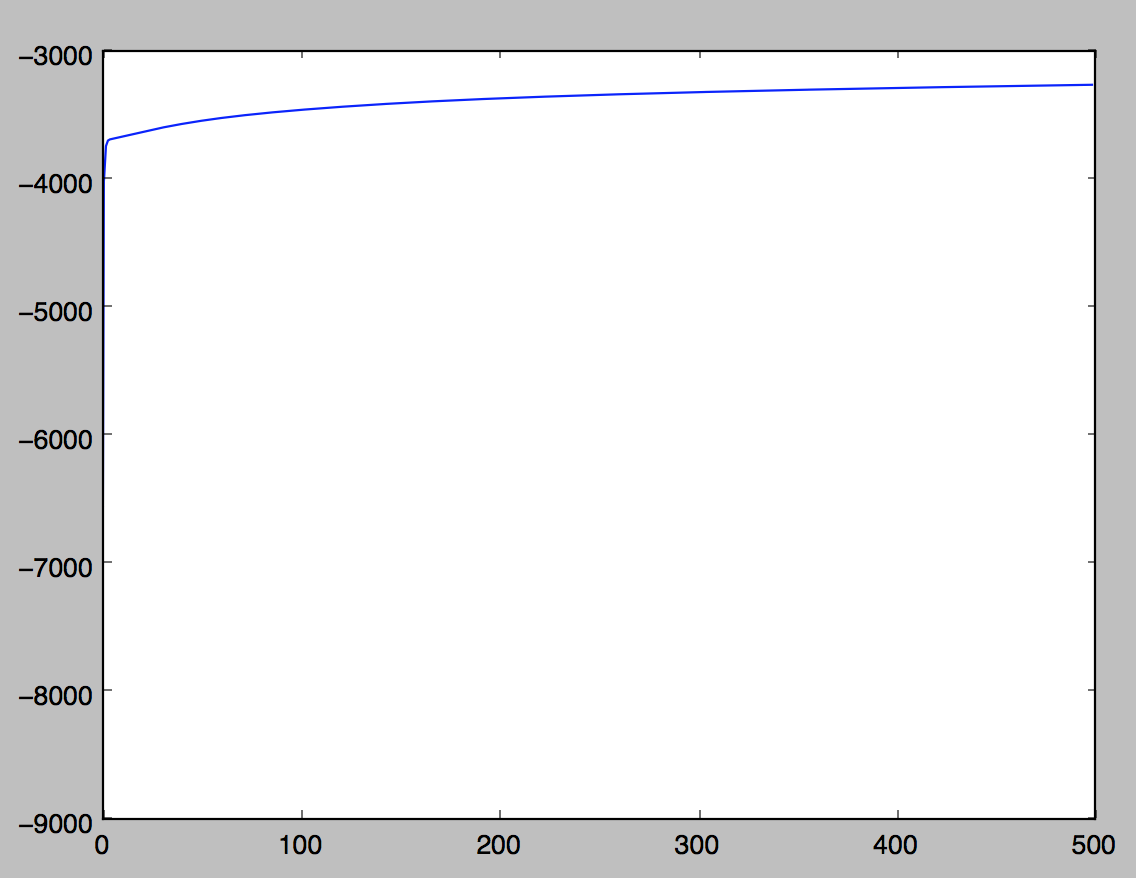
\includegraphics[scale=.5]{images/1objfunc.png}

b. Stem plot of $\frac{1}{\bbE[\alpha_k]}$:

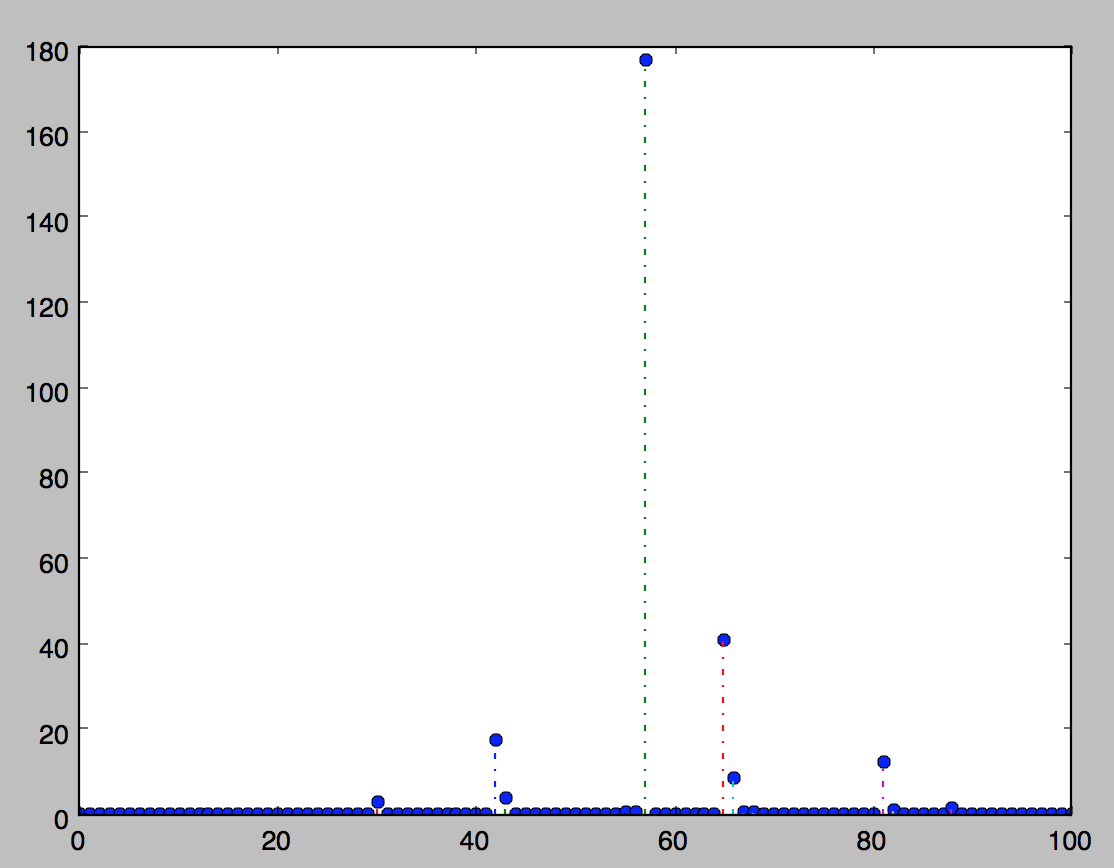
\includegraphics[scale=.5]{images/1stem.png}

c. $\frac{1}{\bbE[\lambda]} = 1.0800299564502283$

d. $\hat{y}$ over $z$:

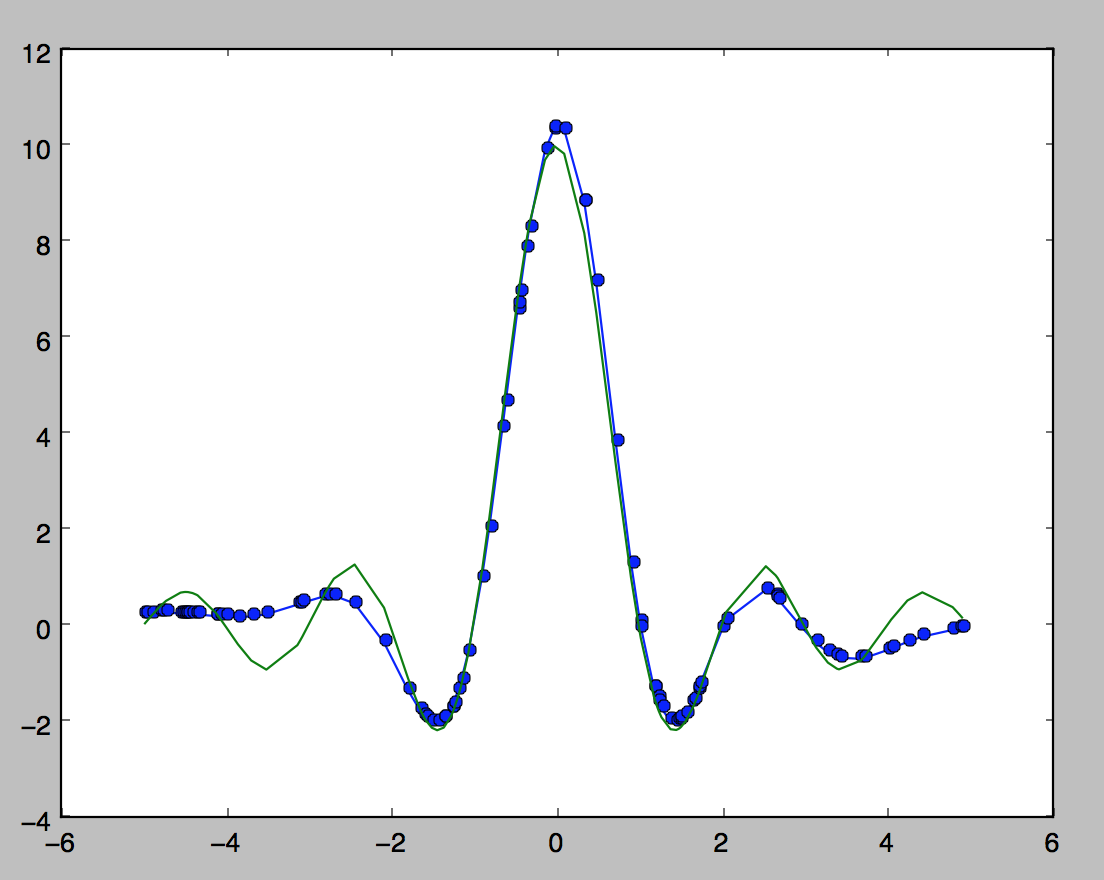
\includegraphics[scale=.5]{images/1yhat.png}

\textbf{N = 250}

a. Variational Objective Function:

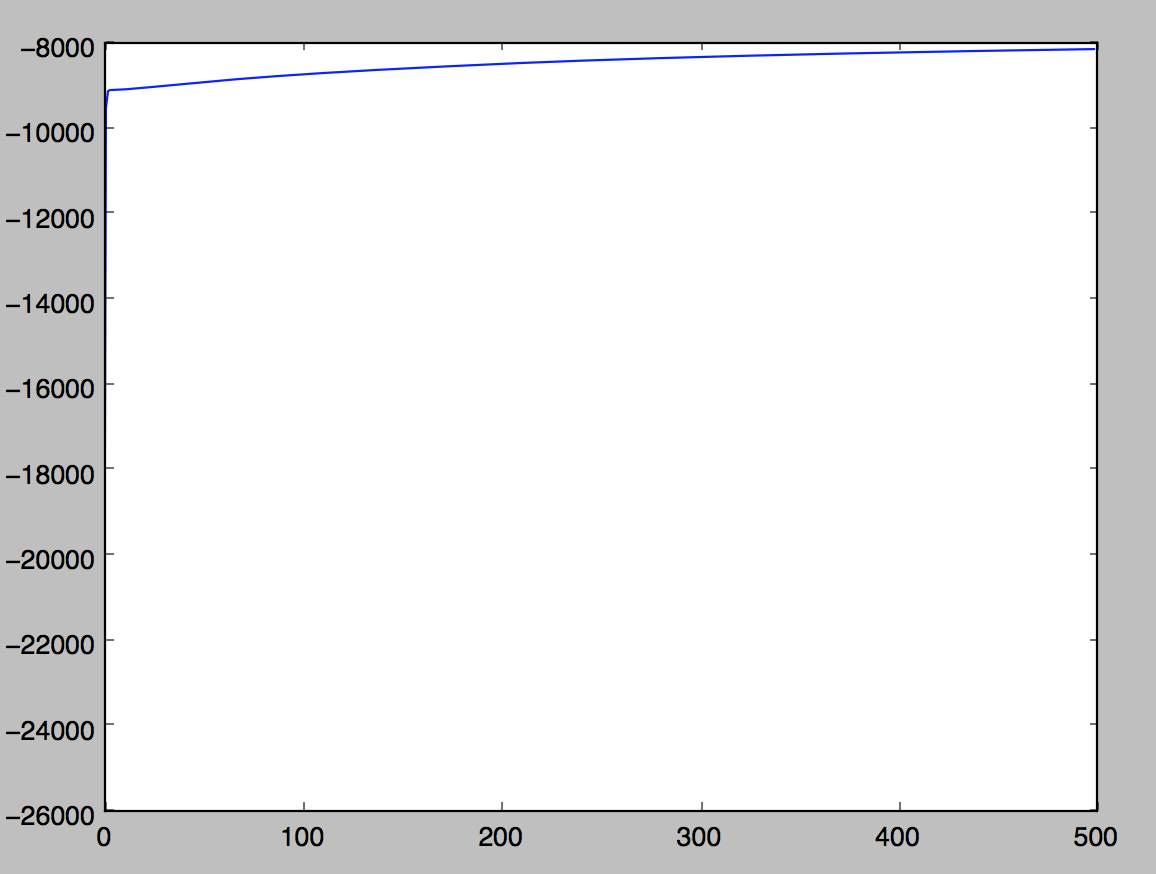
\includegraphics[scale=.5]{images/2objfunc.png}

b. Stem plot of $\frac{1}{\bbE[\alpha_k]}$:

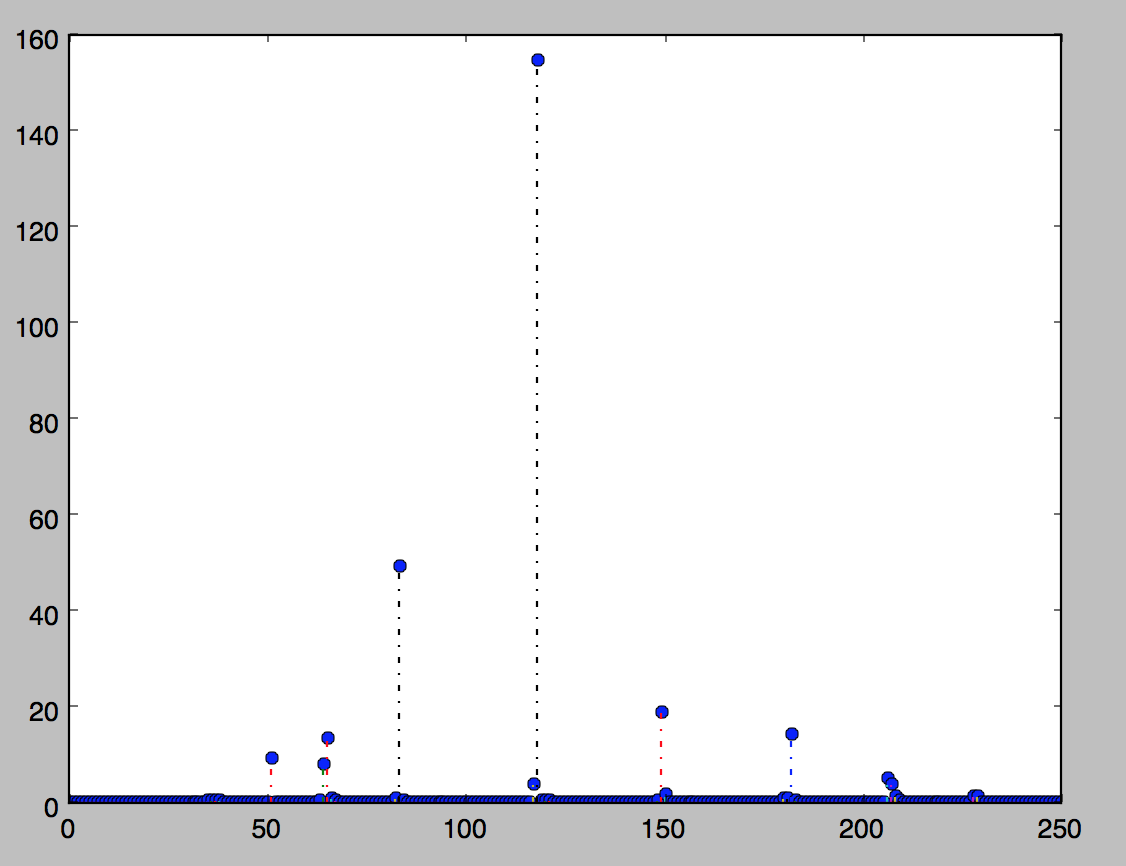
\includegraphics[scale=.5]{images/2stem.png}

c. $\frac{1}{\bbE[\lambda]} = 0.89946298007809866$

d. $\hat{y}$ over $z$:

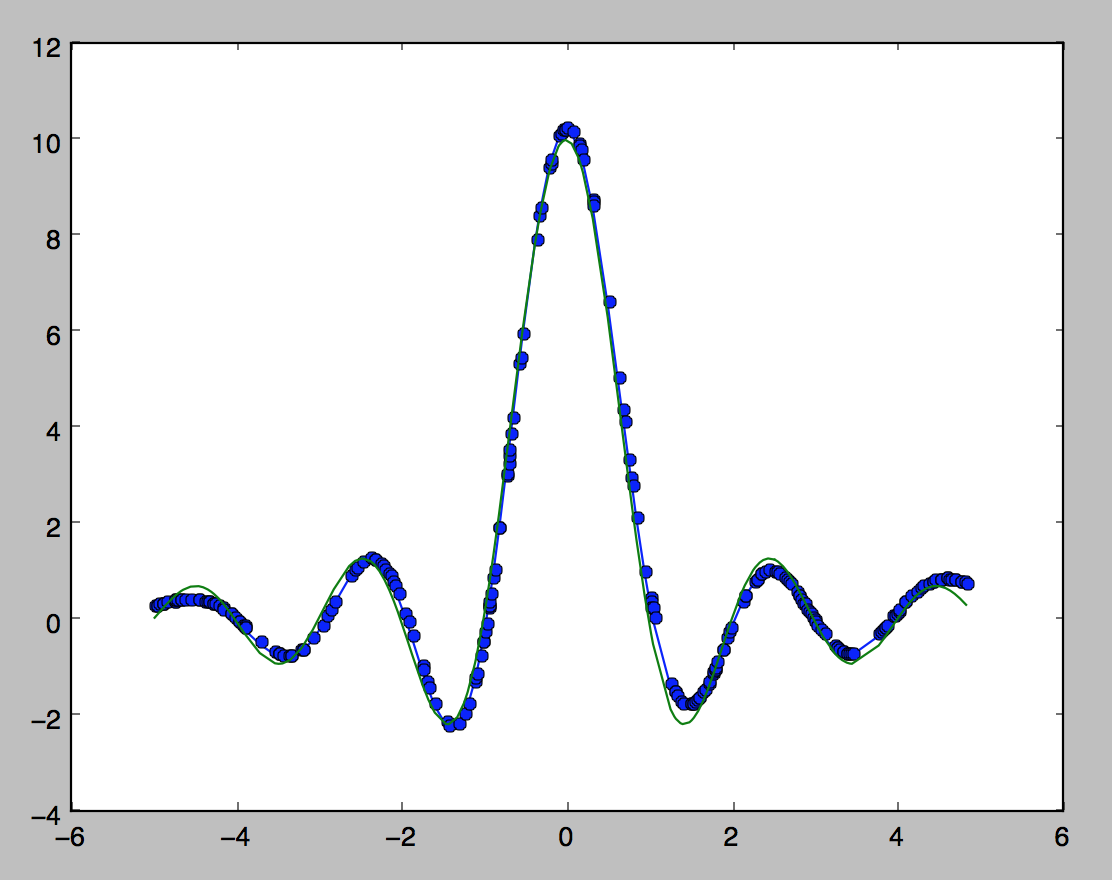
\includegraphics[scale=.5]{images/2yhat.png}


\textbf{N = 500}

a. Variational Objective Function:

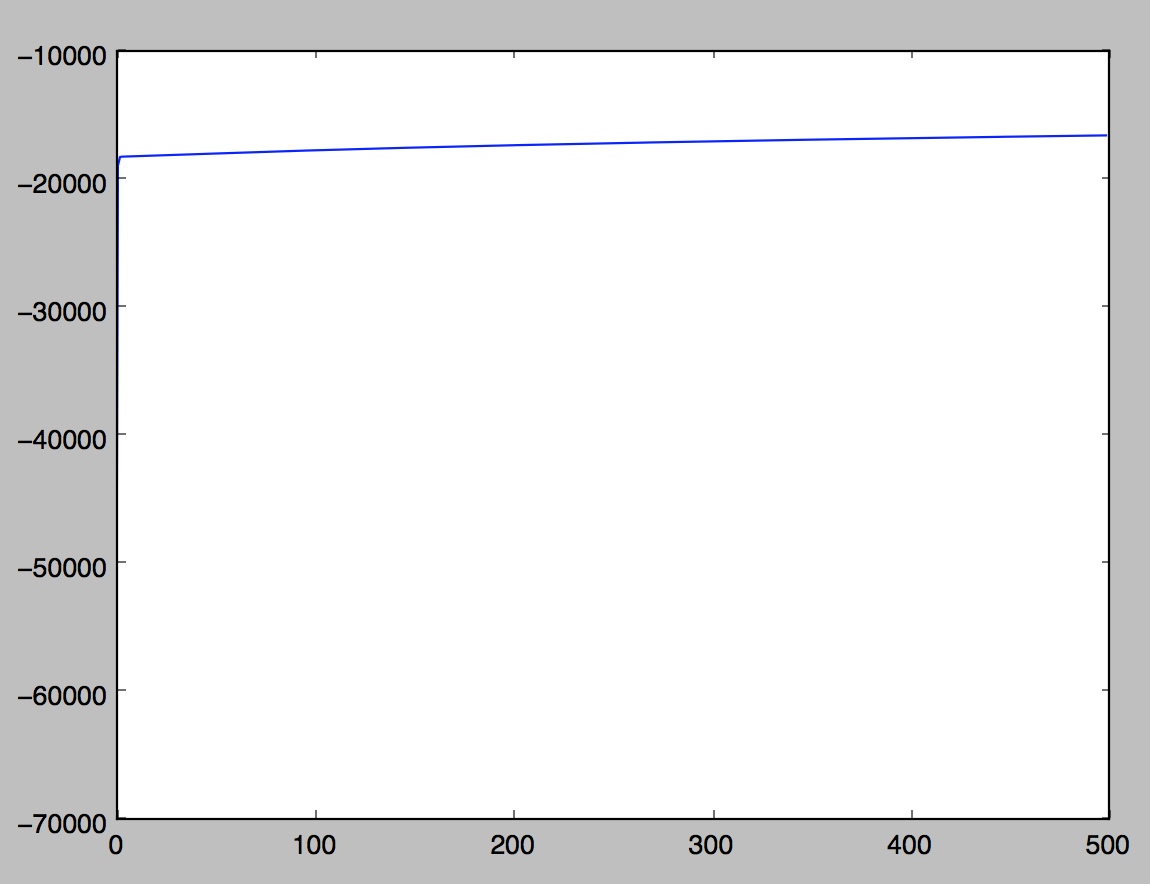
\includegraphics[scale=.5]{images/3objfunc.png}

b. Stem plot of $\frac{1}{\bbE[\alpha_k]}$:

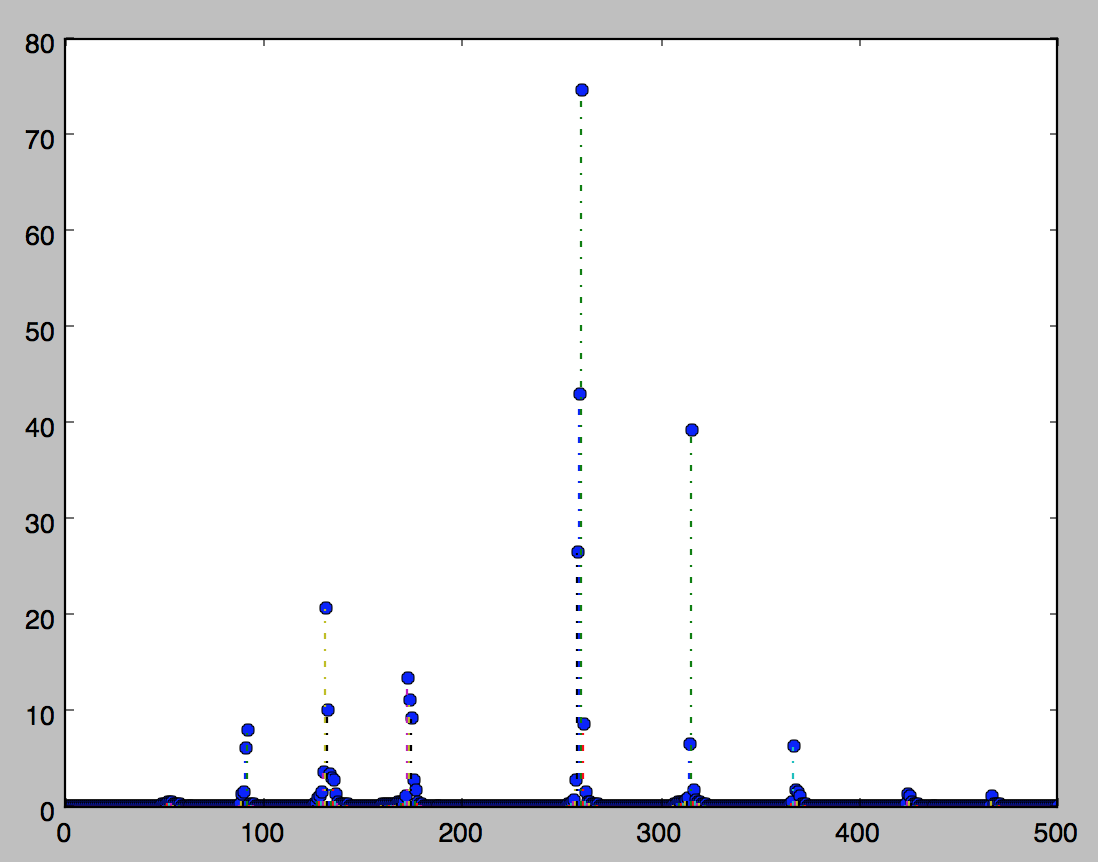
\includegraphics[scale=.5]{images/3stem.png}

c. $\frac{1}{\bbE[\lambda]} = 0.97814359184776878$

d. $\hat{y}$ over $z$:

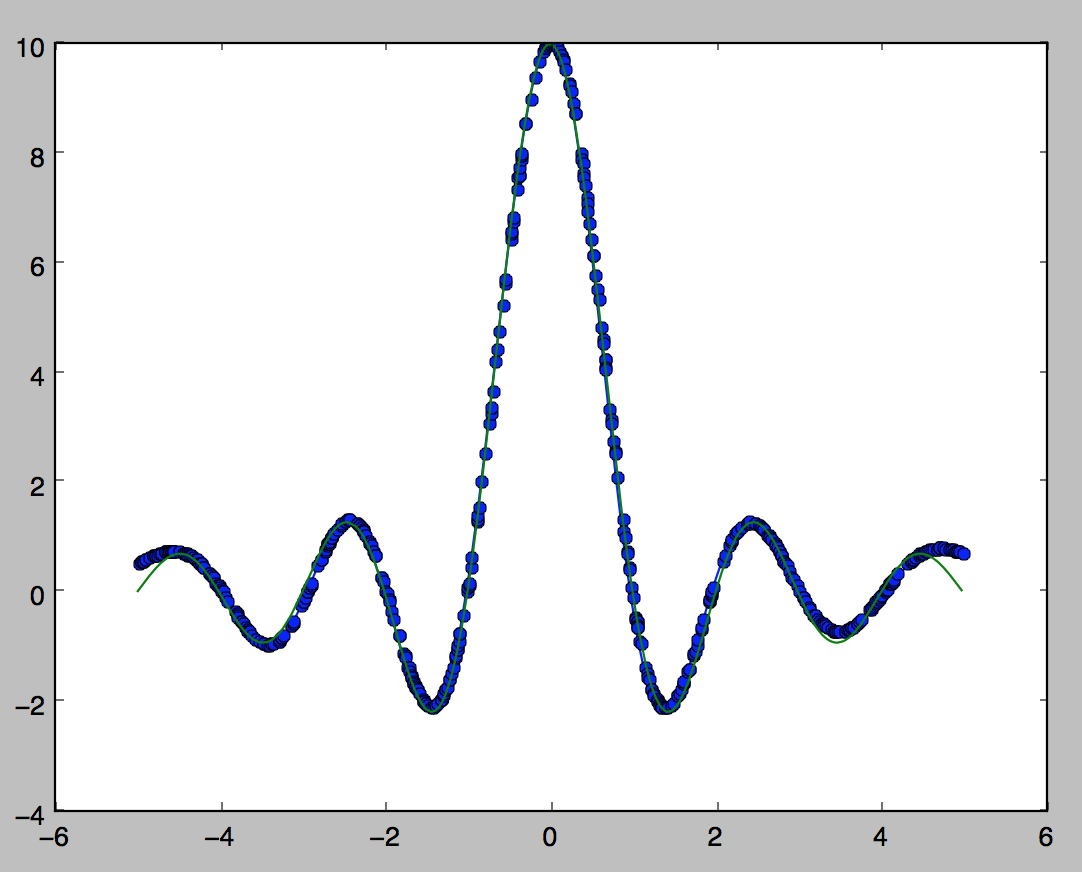
\includegraphics[scale=.5]{images/3yhat.png}

\end{document} 
